\documentclass[11pt,a4paper]{article}

\usepackage[utf8]{inputenc}
\usepackage[brazil]{babel}
\usepackage[protrusion=true, expansion=true]{microtype}
%\usepackage[hang, small, labelfont=bf, up, texfont=it, up]{caption}

\usepackage{graphicx}
\usepackage{epstopdf}
\usepackage{epsfig}
\usepackage{fancyhdr}
\usepackage[ddmmyyyy]{datetime}
\usepackage{lipsum}

\usepackage{hyperref}

\hypersetup{
    colorlinks=true,
    linkcolor=blue,
    filecolor=magenta,      
    urlcolor=cyan,    
    pdfpagemode=FullScreen,
    citecolor=blue,
}

\usepackage{indentfirst} %Primeiro paragrafo identado

\pagestyle{fancy}

\lhead{}
\chead{}
\rhead{}

\lfoot{Relatório 1: Teste em Campo}
\cfoot{}
\rfoot{\footnotsize Folha \thepage\ }

\renewcommand{\headrulewidth}{0.0pt}
\renewcommand{\footrulewidth}{0.3pt}


%\usepackage[hmargin=2cm,vmargin=3.5cm,bmargin=2cm]{geometry}

\title {Relatório 1: Teste em Campo}
\author{Caio Vinícius Ribeiro da Silva}
\date{\today}

\begin{document}

\maketitle

\section{Informações iniciais}

O teste foi realizado no dia 16/04/2022, das 14:11 às 15:49, na região do Parque Villa-Lobos, em São Paulo. A área escolhida, além da sua extensão adequada e do pouco tráfego de pessoas, possui um terreno plano, conforme Figura \ref{fig:area}. O objetivo do teste é verificar o comportamento da transmissão via ESP-NOW entre os emisssores e o receptor nos cenários, alimentado por uma bateria externa e via placa solar.

%\end{center}


\begin{figure}[hbt]
	\centering
		\caption{Área dos testes}
		\includegraphics[width=0.7\textwidth]{LOCAL-2022-4-16} 
%		\\Fonte: Dados do autor
		\label{fig:area} 
\end{figure}



\subsection{Descrição do Hardware}

O Hardware pode ser dividido em duas estações, denominadas Emissora e Receptora. A estação Receptora possui um ESP32 com tela OLED integrada e antena externa, uma shield com um cartão micro SD e um powerbank para alimentação, conforme ilustra a Figura \ref{fig:receptora}. Esse microcontrolador recebe, via protocolo ESP-NOW, os dados das duas placas localizadas na estação Emissora e armazena as informações no cartão micro SD. Além disso, o RTC interno do dispositivo é usado para registrar a hora do recebimento dos dados. 
%
\begin{figure}[hbt]
	\centering
		\caption{Estação receptora}
		\includegraphics[width=0.4\textwidth]{RECEPTORA-2022-4-16} 
		\label{fig:receptora} 

\end{figure} 

A estação Emissora pode ser dividida em dois circuitos. No primeiro há o microcontrolador D1 Mini Pro, que após estabelecer a comunicação com a estação Emissora, envia a palavra ``UFABC", o número 1 e o valor do RSSI. Após 1 segundo, o dispositivo continua enviando a mesma palavra, mas incrementa o número para 2, e atualiza o valor do RSSI, repetindo o processo enquanto houver comunicação. A alimentação desse circuito pode ser via energia do powerbank ou energia solar, captada pelo kit de desenvolvimento solar, composto por uma placa solar, uma bateria de 3,7V/40mAh e o circuito integrado gerenciador de energia solar. A Figura \ref{fig:emissora} apresenta a disposição da estação Emissora.

\begin{figure}[hbt]
	\centering
		\caption{Estação Emissora}
		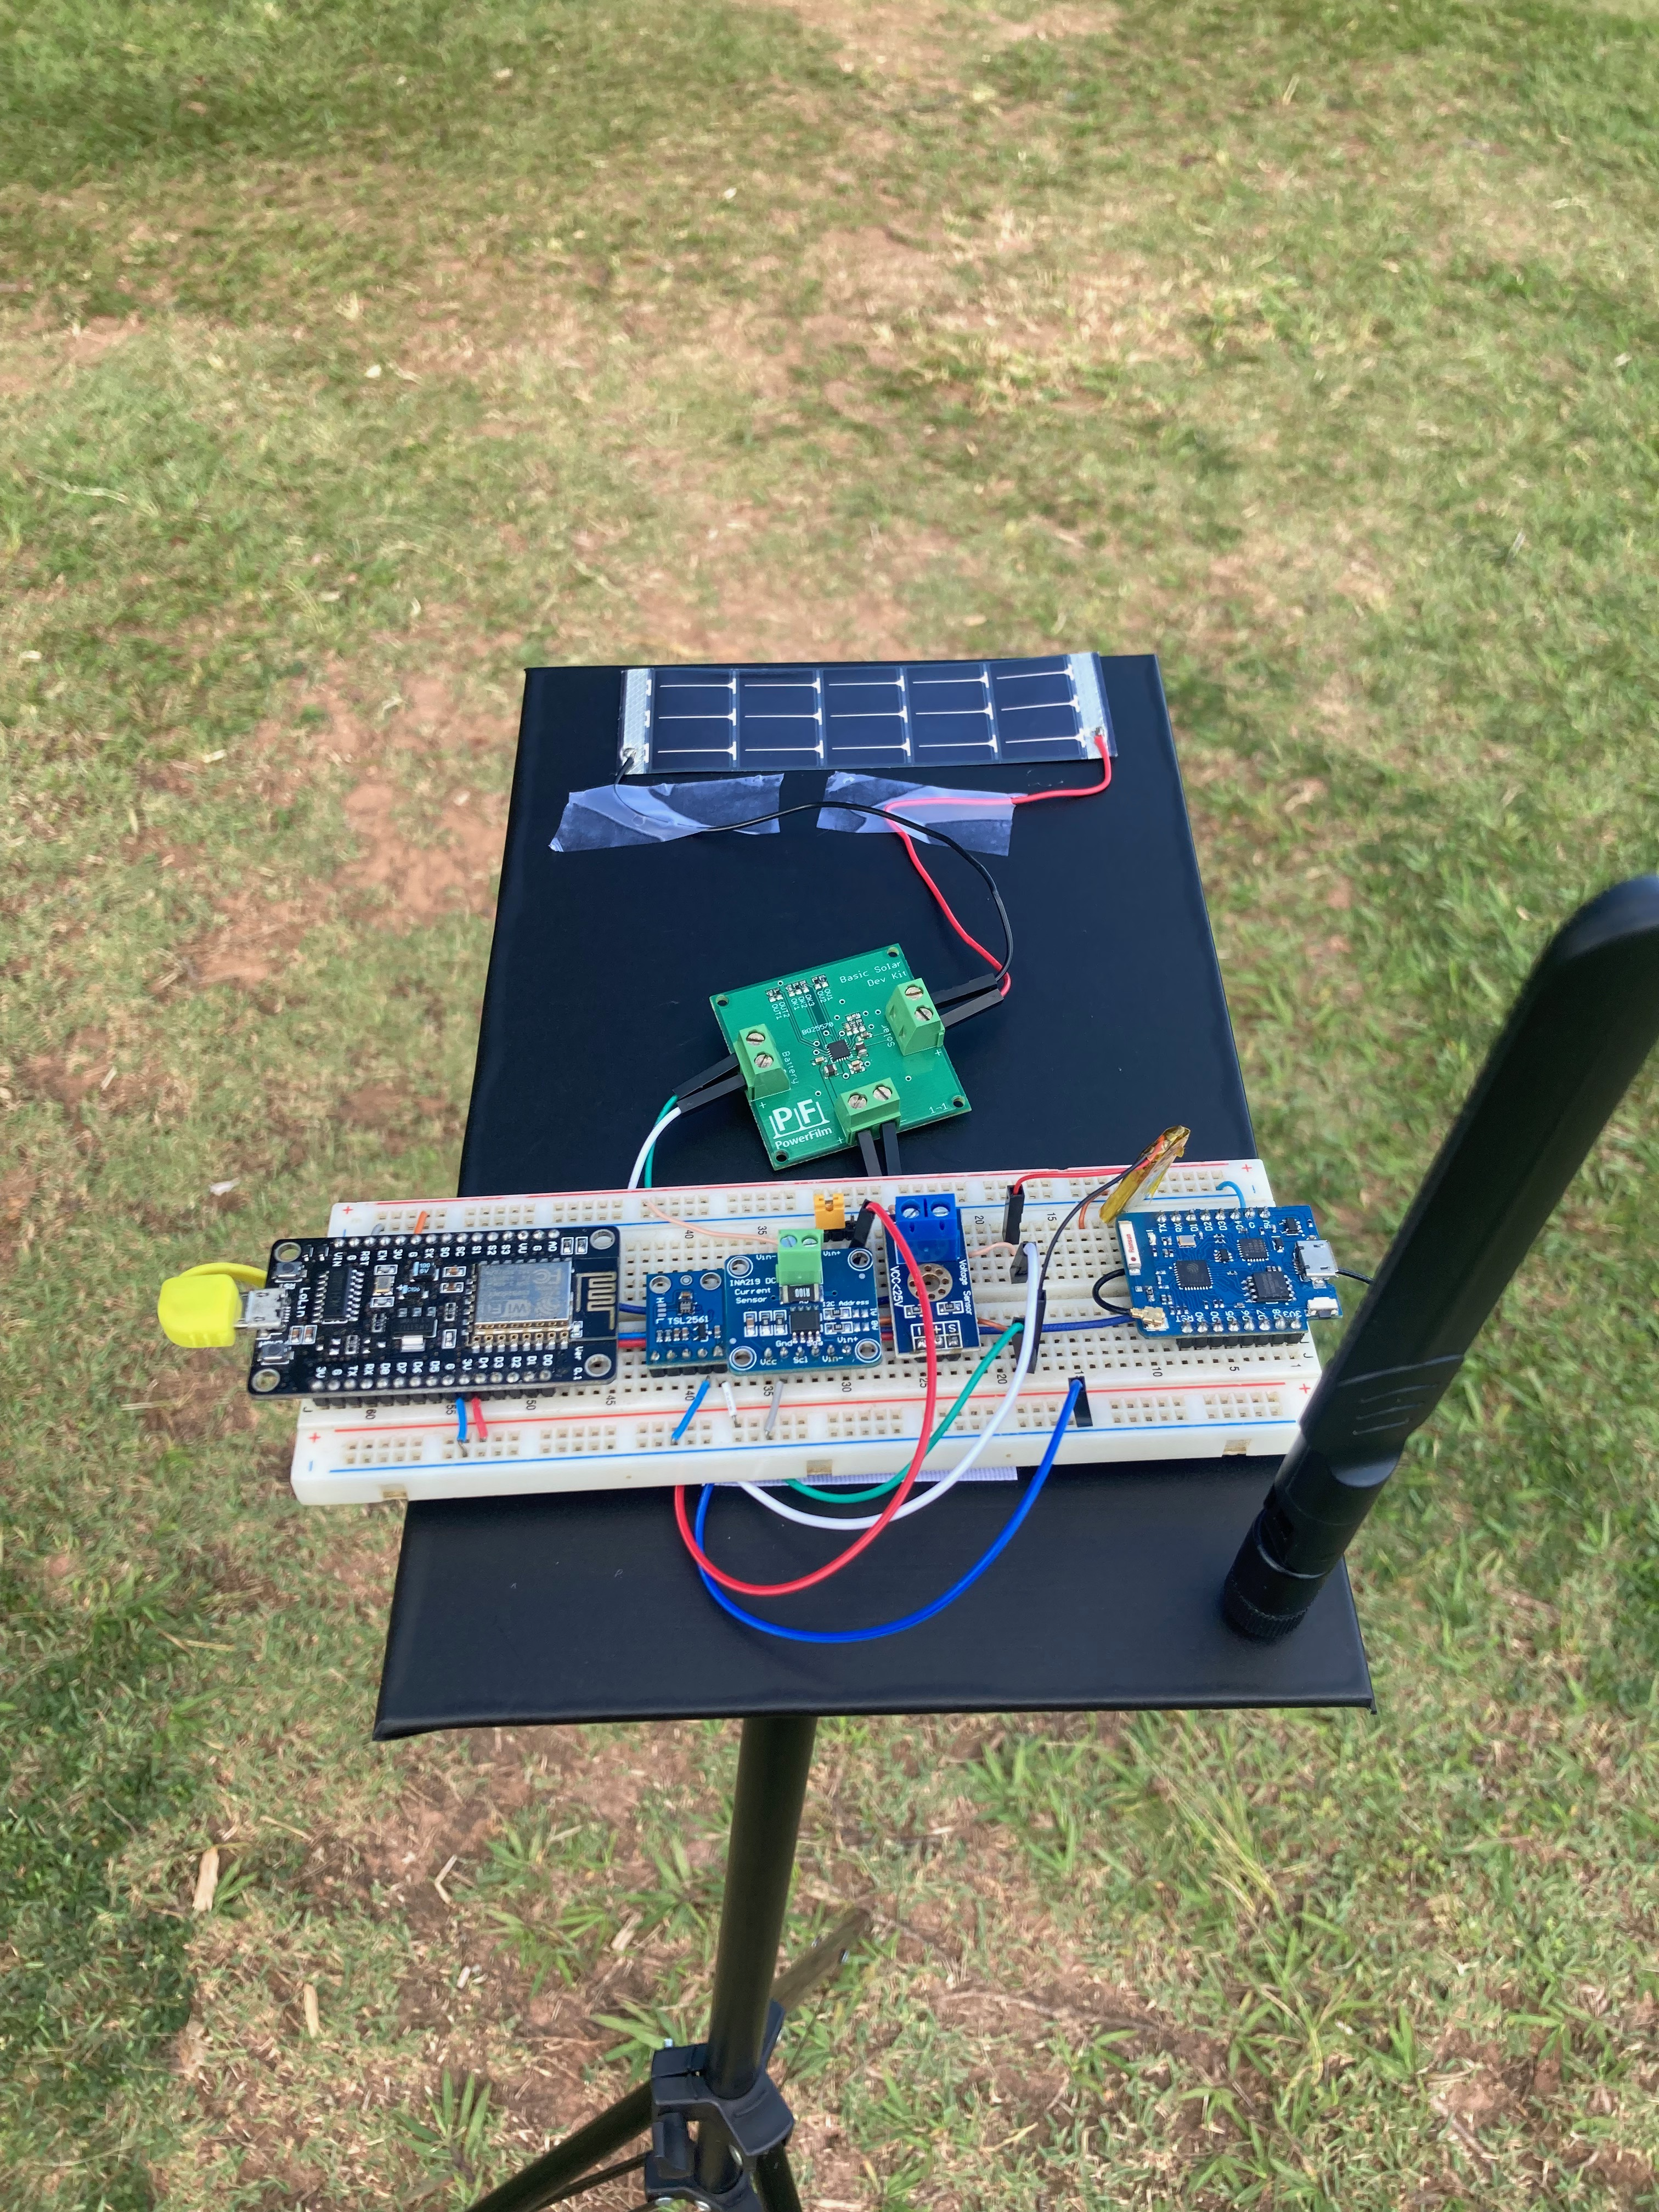
\includegraphics[width=0.4\textwidth]{EMISSORA-2022-4-16} 
%		\\Fonte: Dados do autor
		\label{fig:emissora} 
\end{figure} 


O segundo circuito é composto pelo microcontrolador NodeMCU, sensor de luminosidade, dois medidores de tensão elétrica, um medidor de corrente elétrica. O dispositivo coleta os dados de tensão elétrica, corrente elétrica do D1 Mini Pro, capta a luminosidade do ambiente via sensor e envia os dados, também via ESP-NOW para a placa Receptora. Esse circuito é usado apenas para medir os dados  de consumo e luminosidade. 

Cada uma das estações foi disposta em um tripé, como o objetivo de acomodar os dispositivos, facilitar o transporte e padronizar a altura em relação ao solo, como pode ser visto na Figura \ref{fig:emissorareceptora}. Para o presente teste, foi adotada a altura de 1 metro em relação ao solo.

\begin{figure}[hbt]
	\centering
		\caption{Estação Receptora e Emissora}
		\includegraphics[width=0.5\textwidth]{EMISSORA-RECEPTORA-2022-4-16} 
%		\\Fonte: Dados do autor
		\label{fig:emissorareceptora} 
\end{figure}  



\section{Dados coletados}

O teste foi realizado no dia 16/04/2022, das 14:11 às 15:49. Os dados foram armazenados em um arquivo csv, com 5643 entradas, dispostos conforme Tabela \ref{tab:dados}. A tabela apresenta as primeiras cinco medições, que estão com o valor zero porque a estação Emissora ainda não havia sido ligada.

\begin{table}[!ht]\footnotesize


\caption{Estrutura do dados coletados}
\label{tab:dados}

\begin{tabular}{ccccccccc}
\hline
\textbf{datetime} & \textbf{ID} & \textbf{VD1(V)} & \textbf{ID1(A)} & \textbf{VBAT(V)} & \textbf{lux} & \textbf{RSSI} & \textbf{STRING} & \textbf{N} \\ \hline
\textbf{14:11:02} & 1           & 0               & 0               & 0                & 0            & 0             &                 & 0          \\ \hline
\textbf{14:11:03} & 2           & 0               & 0               & 0                & 0            & 0             &                 & 0          \\ \hline
\textbf{14:11:04} & 3           & 0               & 0               & 0                & 0            & 0             &                 & 0          \\ \hline
\textbf{14:11:05} & 4           & 0               & 0               & 0                & 0            & 0             &                 & 0          \\ \hline
\textbf{14:11:06} & 5           & 0               & 0               & 0                & 0            & 0             &                 & 0          \\ \hline
\end{tabular}
\end{table}


Sobre as colunas:
\begin{itemize}
  \item datetime: hora que a informação é salva, ação realizada a cada 1 segundo; 
  \item ID: é incrementado quando os dados são salvos no cartão de memória. Caso haja um problema no registro dos dados, ele será rapidamente identificado porque a sequência será rompida;
  \item VD1(V): tensão elétrica do D1 Mini Pro, enviada pelo NodeMCU;
  \item ID1(A): corrente elétrica do D1 Mini Pro, enviada pelo NodeMCU;
  \item VBAT(V): tensão elétrica da bateria, conectada no kit solar;
  \item lux: luminosidade do ambiente, enviada pelo NodeMCU;
  \item RSSI: enviado pelo D1 Mini Pro, apresenta o valor da conexão com a estação Receptora em decibéis;
  \item STRING: palavra ``UFABC", enviada pelo D1 Mini Pro;
  \item N: quando o microcontrolador D1 Mini Pro se conecta com a estação receptora, inicia a transmissão do número 1 a cada 1 segundo, incrementa e envia o novo valor. Quando a Estação Receptora não recebe o valor do emissor, salva o número 0 nesse campo.
\end{itemize}

\section{Procedimentos e resultados}

O teste foi dividido em duas partes: na primeira, a alimentação da placa D1 Mini Pro foi através de um powerbank e o objetivo foi verificar a transmissão de dados e a máxima distância sem queda de conexão. Na segunda parte, a placa D1 Mini Pro foi alimentada via kit de desenvolvimento solar, apresentado na Figura \ref{fig:kitsolar1}.

\begin{figure}[hbt]
	\centering
		\caption{Disposição do Kit Solar}
		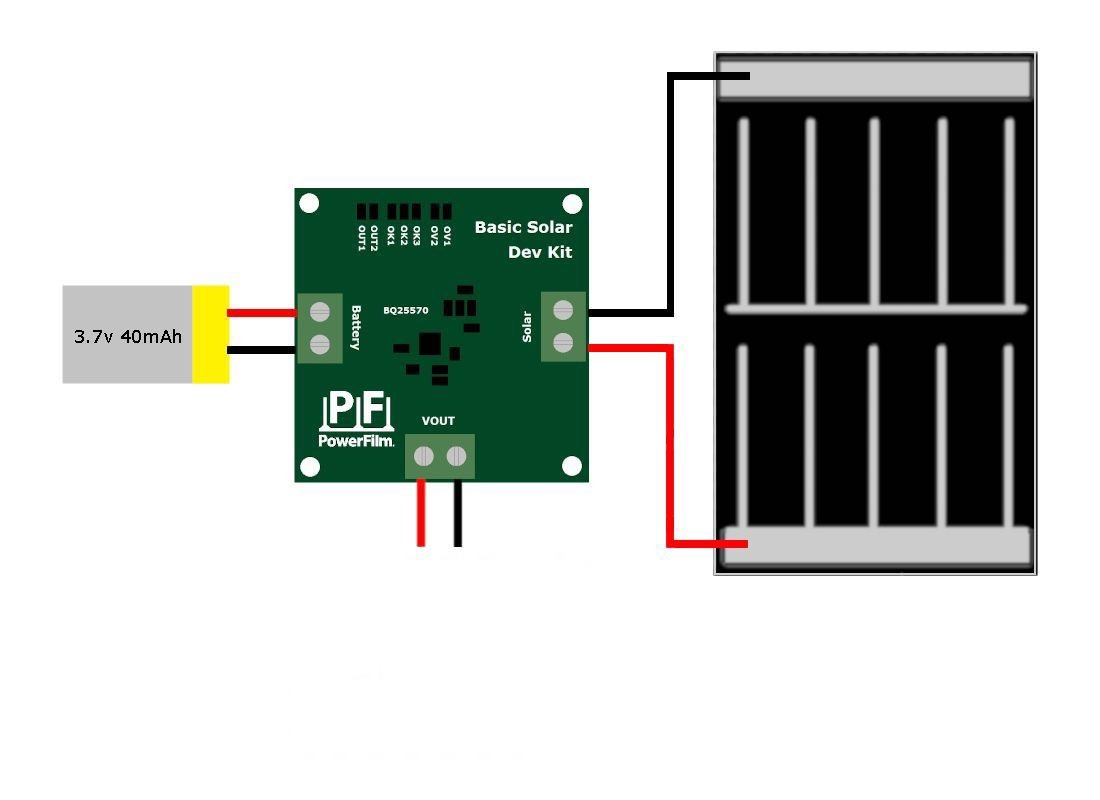
\includegraphics[width=0.7\textwidth]{kitsolar1.jpg} 
		\label{fig:kitsolar1} 
\end{figure}  


\subsection{Parte 1 - Teste com alimentação via Kit Solar}

A partir das 14:48 foi realizada a troca de alimentação do microcontrolador D1 Mini Pro, que antes estava conectada na bateria externa e a partir desse momento foi conectada na saída VOUT do kit solar, conforme conexão apresentada na Figura \ref{fig:kitsolar1}. Aos 50m, a conexão ficou estável, com os dados transmitidos



Como pode ser observado na Figura \ref{fig:dadoskit}, no momento da substituição da alimentação, a tensão elétrica que antes estava em 3,3V cai para 1,7V. Além disso, a tensão da bateria do kit, representada por VBAT apresentou 0,96V durante todo o período de testes e não foi carregada pela célula solar. Antes, a bateria foi carregada para atingir a tensão nominal de 3,3V, mas isso não ocorreu. Ainda no momento da troca de fonte de energia, a corrente elétrica sobe de 18mA para 140mA, conforme ilustra a Figura \ref{fig:id1}. 


\begin{figure}[hbt]
	\centering
		\caption{Dados coletados durante conexão com kit solar}
		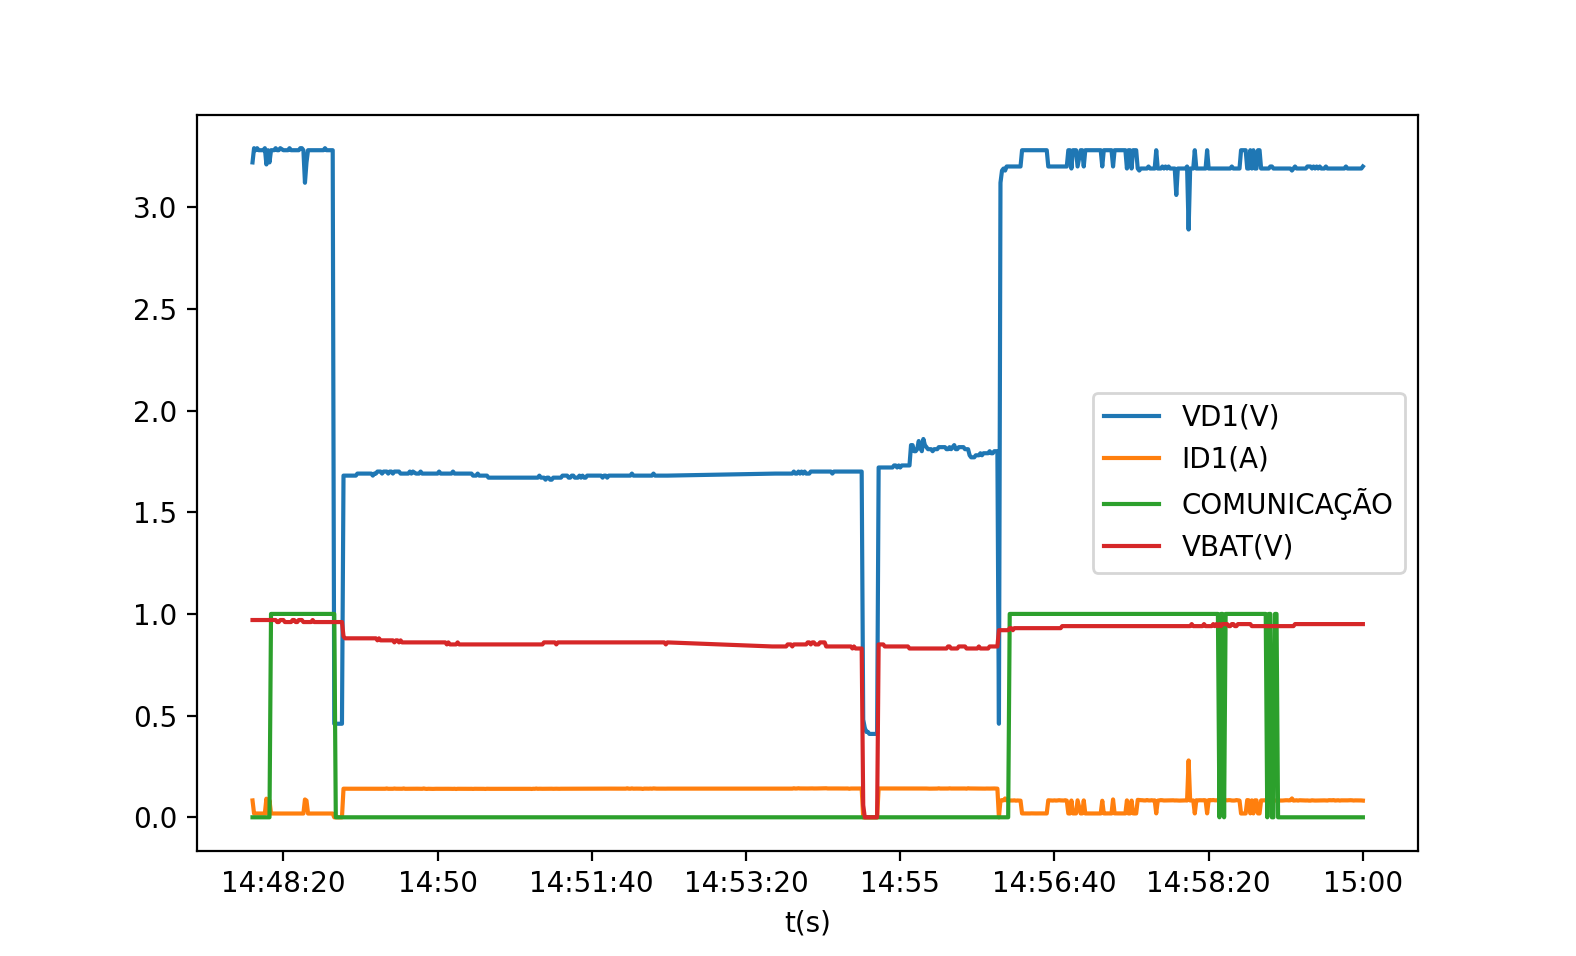
\includegraphics[width=0.8\textwidth]{gsolar.png} 
		\label{fig:dadoskit} 
\end{figure} 
 
\begin{figure}[hbt]
	\centering
		\caption{Mudança da corrente elétrica}
		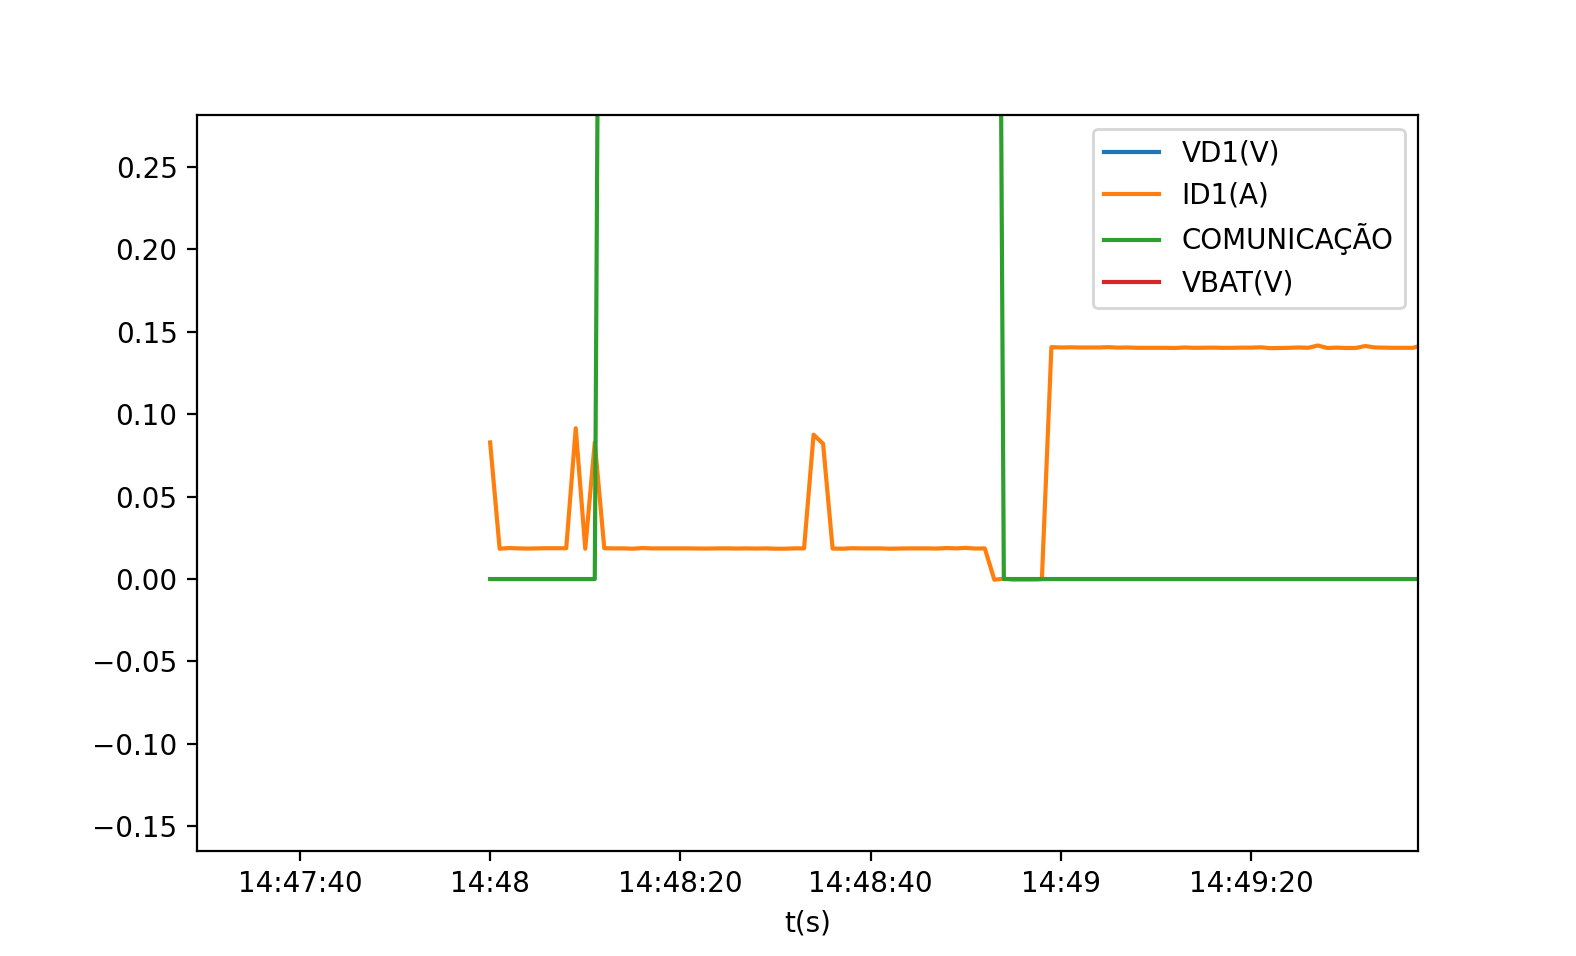
\includegraphics[width=0.8\textwidth]{gsolarID1.png} 
		\label{fig:id1} 
\end{figure} 

\begin{figure}[hbt]
	\centering
		\caption{Retirada da bateria do kit solar}
		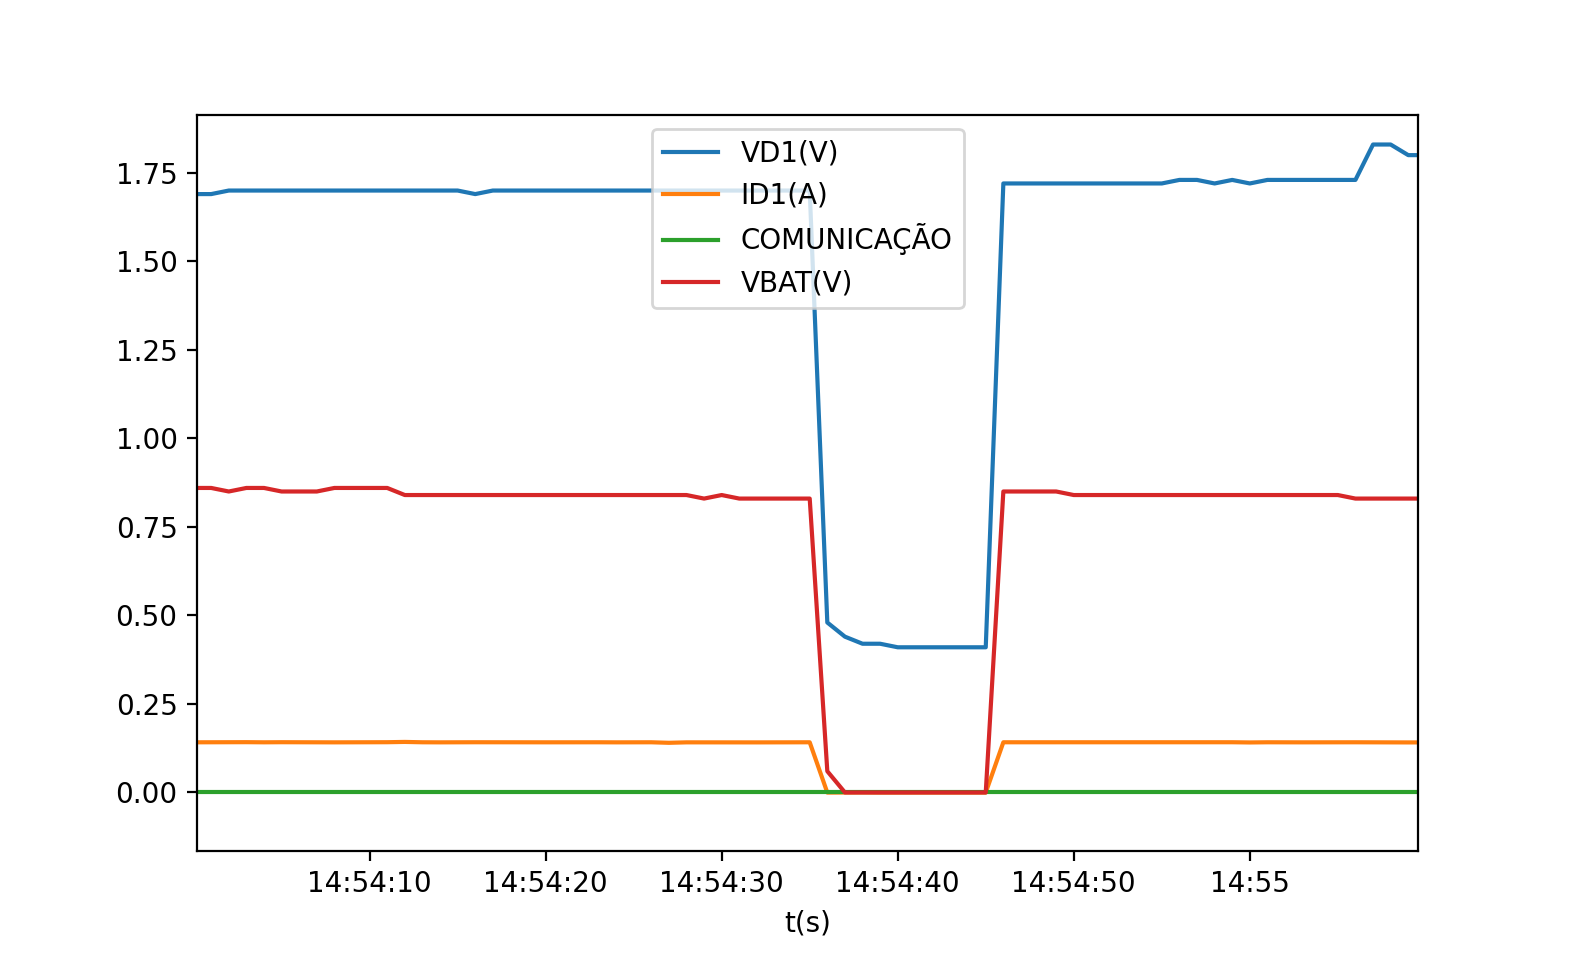
\includegraphics[width=0.8\textwidth]{gsolarVBAT.png} 
		\label{fig:VBAT} 
\end{figure}

Para facilitar a interpretação, os dados de comunicação foram convertidos para a forma binária, de modo que o número 1 indica conexão e o 0 indica a sua desconexão, que podem ser identificados na Figura \ref{fig:dadoskit}. Quando é feita a troca da alimentação, a conexão é perdida e o microcontrolador não tem potência elétrica o suficiente para realizar a conexão. No horário 14:54 a bateria do kit é retirada e o valor de VBAT cai para zero, conforme ilustra a Figura \ref{fig:VBAT}. A célula solar forneceu apenas 0,4V sem a existência de corrente elétrica. Portanto, conclui-se que a bateria e a célula solar não estavam fornecendo potencia suficiente para alimentar o circuito. Como não foi possível fazer a leitura da luminosidade ambiente, o resultado no momento, carece de mais testes e ajustes, que serão discutidos na seção \ref{sec:ajustes}. 


\subsection{Parte 2 - Teste com alimentação externa}

A partir das 15:13 foi iniciado o distanciamento de 50m, mantendo a comunicação estável em 50m de distância. No instante 15:29, a comunicação do D1 Mini Pro é perdida em 80m, conforme apresenta a Figura \ref{fig:50m}.

\begin{figure}[hbt]
	\centering
		\caption{Transmissão com alimentação externa}
		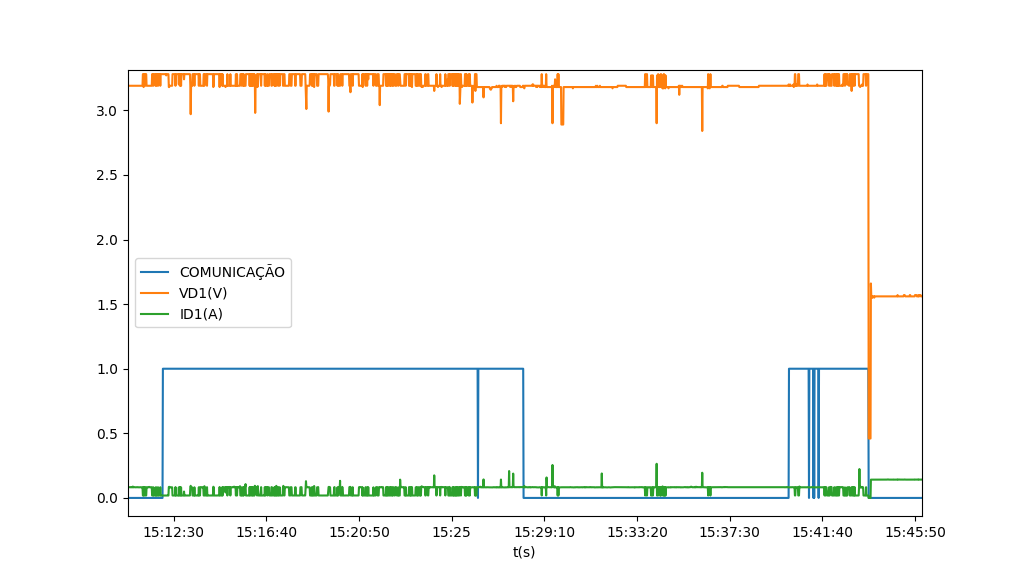
\includegraphics[width=0.9\textwidth]{powerbank50m.png} 
		\label{fig:50m} 
\end{figure} 

\newpage

Todavia, os dados da tensão VD1 e ID1 ainda são recebidos, via nodeMCU. A comunicação só é perdida no instante 15:43, quando é feito um teste com alimentação via kit solar. Em resumo, a alimentação via powerbank apresentou um resultado satisfatório, com um fato relevante: com a distância de 80m houve a perda da comunicação do D1 Mini Pro, que possui antena externa, mas só após 153 m que ocorreu a perda da comunicação do nodeMCU, que não tem antena. Esses resultados serão discutidos na próxima secão.


\subsection{Ajustes necessários}
\label{sec:ajustes}

A leitura da luminosidade apresentou problemas. Nos testes internos, não houve erros devido à baixa luminosidade. Entretanto, como houve alto índice de luminosidade na data do teste, ocorreu um problema na leitura e o microcontrolador acabou registrando o valor zero, devido ao fim de escala. Após pesquisa, foi constatado que é necessário fazer um ajuste no ganho do sensor para ambientes com alta luminosidade. O ajuste foi feito e será verificado no próximo teste outdoor.

Outro empecilho foi a conexão do microcontroldador D1 Mini Pro. Os dois microcontroladores localizados na estação Emissora enviam os dados via ESP-NOW, com a diferença que o D1 possui antena externa. A suposição antes do teste é que ele conseguiria enviar os dados em maior distância, mas na prática não foi isso que aconteceu. Ele perdia comunicação mais rápido que o NodeMCU, sem a antena.

O protocolo ESP-NOW não exige uma conexão constante. Os emissores apenas enviam a informação para o endereço MAC cadastrado, de modo que não é necessário manter a conexão. Entretanto, para obter o RSSI, foi criado um Access Point no Receptor, sendo realizada a conexão usando o D1 Mini Pro. Só depois que a conexão é feita que o microcontrolador envia os dados, limitando o alcance dos dados. Uma alternativa de solução é eliminar essa conexão e enviar os dados apenas usando o protocolo ESP-NOW, sem a conexão na estação receptora. Isso implica na ausência do valor de RSSI.

\section{Considerações finais e próximas ações}

O objetivo de estabelecer a comunicação entre as estações foi alcançado. Muitos dos problemas do hardware, como comunicação, ajuste de dados do RTC, gravação dos dados no cartão, entre outros, foram solucionados.

Entretanto, o kit solar não forneceu a alimentação, conforme descrito pelo fabricante, e a não aquisição da luminosidade impede de calcular qual deveria ser a tensão oferecida pela célula solar. Foi feita a compra de outra bateria com as mesmas características e o ajuste do ganho do sensor de luminosidade foi corrigido, via programação. O próximo teste oferecerá a oportunidade de verificar essas modificações.


\end{document}